\documentclass{article}
\usepackage[spanish, es-tabla]{babel}
\usepackage[utf8]{inputenc}
\usepackage{amsmath, amsthm, amsfonts}
\usepackage{graphicx}
\usepackage{cite}
\usepackage{float}
%\usepackage{listings}
\usepackage{tabularx}
%\usepackage{multirow}
\usepackage{colortbl}
%\renewcommand{\refname}{Referencias}
\usepackage{subfig}
\usepackage{booktabs}
\usepackage{cite}
\usepackage[makeroom]{cancel}

\usepackage[utf8]{inputenc}
\usepackage[english]{babel}

\usepackage{hyperref}
\hypersetup{
    colorlinks=true,
    linkcolor=blue,
    filecolor=magenta,      
    urlcolor=cyan,
}

\urlstyle{same}

\usepackage[
    papersize={21.7cm,27.9cm},
    top=2.54cm,
    bottom=2.54cm,
    left=2.54cm,
    right=2.54cm
]{geometry}

\renewcommand{\citedash}{ -- } 

\renewcommand{\tablename}{\small{\textsc{Tabla}}}

\usepackage{xcolor}
\usepackage{listings}
\definecolor{codegray}{rgb}{0.5,0.5,0.5}
\definecolor{backcolour}{rgb}{0.66,0.66,0.66}
\definecolor{darkpastelgreen}{rgb}{0.01, 0.75, 0.24}
\definecolor{electricgreen}{rgb}{0.0, 1.0, 0.0}
\definecolor{gainsboro}{rgb}{0.86, 0.86, 0.86}
\definecolor{bostonuniversityred}{rgb}{0.8, 0.0, 0.0}

\lstdefinestyle{mystyle}{
    backgroundcolor=\color{gainsboro},   
    commentstyle=\color{yellow},
    keywordstyle=\color{bostonuniversityred},
    numberstyle=\tiny\color{black},
    stringstyle=\color{blue},
    basicstyle=\ttfamily\footnotesize,
    breakatwhitespace=false,         
    breaklines=true,                 
    captionpos=b,                    
    keepspaces=true,                 
    numbers=left,                    
    numbersep=5pt,                  
    showspaces=false,                
    showstringspaces=false,
    showtabs=false,                  
    tabsize=2,
    morekeywords = [2]{sudo,chmod,touch,scp,ssh,ls,ls -l,mkdir,mv,make,cmake,apt,install,df,-h,chown,cd,which},
    keywordstyle = [2]\color{bostonuniversityred}
}


\lstdefinestyle{mystyle2}{
    backgroundcolor=\color{gainsboro},   
    commentstyle=\color{yellow},
    %keywordstyle=\color{bostonuniversityred},
    numberstyle=\tiny\color{black},
    stringstyle=\color{blue},
    basicstyle=\ttfamily\footnotesize,
    breakatwhitespace=false,         
    breaklines=true,                 
    captionpos=b,                    
    keepspaces=true,                 
    numbers=left,                    
    numbersep=5pt,                  
    showspaces=false,                
    showstringspaces=false,
    showtabs=false,                  
    tabsize=2
   % morekeywords = [2]{sudo,make,cmake},
   %keywordstyle = [2]\color{bostonuniversityred}
}




\begin{document}

\begin{titlepage}
    \centering
    %{\includegraphics[width=0.2\textwidth]{logo}\par}
    %\vspace{1cm}
    %{\bfseries\LARGE Título del proyecto \par}
    %\vspace{1cm}
    %{\scshape\Large Facultad de Ingenier\'ia Industrial \par}
    \vspace{4cm}
    {\scshape\Huge Manual de implementación de un esquema de computación distribuida para Geant4 \par}
    \vspace{3cm}
  {\itshape\Large Grupo de Física Nuclear \par}
    \vfill
    {\Large Autor: \par}
     \vspace{0.5cm}
    {Wilson Javier Almario Rodriguez.}\\
    \vfill
    {\Large Universidad Nacional De Colombia \par}
    {\Large Grupo de física nuclear \par}
    {\Large Bogota, Colombia \par}
    {\Large Junio 2020 \par}
    
\end{titlepage}


\tableofcontents

\clearpage

%\section{Pasos para Paralelizar un programa en Geant4}


\begin{enumerate}
    \item Hacer hostst/cluster del entorno MPI 
    \item Lanzar el entorno de ejecución de MPI.
    \item Ejecutar aplicación mpirun -n # <your application>
    \item Ejecutar comandos MPI G4UI, ubicados en /mpi/
    
\end{enumerate}


\newpage

\section{Introducción}
\subsection{Conceptos claves}

\subsubsection{Computación Paralela}

La computación paralela es el uso simultáneo de más de un procesador para resolver
un problema.
La computación paralela es una técnica de programación en la que muchas instrucciones se ejecutan simultáneamente. Se basa en el principio de que los problemas grandes se pueden dividir en partes más pequeñas que pueden resolverse de forma concurrente.

\subsubsection{MPI}
MPI es un estándar de programación en paralelo mediante paso
de mensajes que permite crear programas portables y eficientes.
El paso de mensajes es una técnica empleada en programación concurrente para aportar sincronización entre procesos y permitir la exclusión mutua.

Su principal característica es que no precisa de memoria compartida, por lo que es muy importante en la programación de sistemas distribuidos. 

Al arrancar una aplicación se lanzan en paralelo n copias del mismo programa(procesos), facilita legibilidad y mantenimiento Distinción del código a ejecutar por cada uno: mediante el id del proceso

\begin{figure}[H]
    \centering
  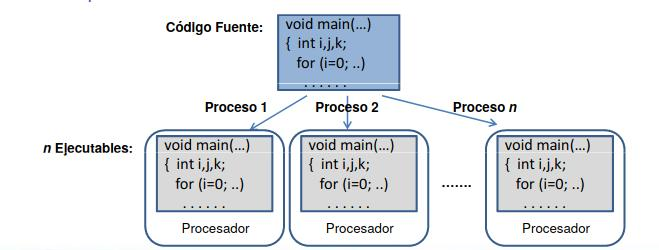
\includegraphics[width=0.7\textwidth]{images/mpi_estructure.jpg}
  \caption{Estructura MPI}
  \label{esq}
\end{figure}


\subsubsection{NFS}

El Sistema de archivos de red (NFS) es una aplicación cliente / servidor que permite al usuario de una computadora ver y opcionalmente, almacenar y actualizar archivos en una computadora remota como si estuvieran en la computadora del usuario. El protocolo NFS es uno de los varios estándares del sistema de archivos distribuidos para el almacenamiento conectado a la red (NAS).

NFS permite al usuario o administrador del sistema montar (designar como accesible) todo o una parte de un sistema de archivos en un servidor. Los clientes pueden acceder a la parte del sistema de archivos que está montada con los privilegios asignados a cada archivo (solo lectura o lectura-escritura). NFS utiliza llamadas a procedimiento remoto (RPC) para enrutar solicitudes entre clientes y servidores. \url{https://searchenterprisedesktop.techtarget.com/definition/Network-File-System}

\subsubsection{Geant4}
Geant4 es un conjunto de herramientas para la simulación del paso de partículas a través de la materia. Sus áreas de aplicación incluyen física de alta energía, nuclear y aceleradora, así como estudios en medicina y ciencia espacial.

\subsubsection{G4mpi}

G4MPI es una interfaz nativa con bibliotecas MPI. El directorio contiene una biblioteca Geant4 UI y un par de ejemplos paralelos. Al usar esta interfaz, las aplicaciones de los usuarios se pueden paralelizar con diferentes bibliotecas compatibles con MPI, como OpenMPI, LAM / MPI, MPICH2, etc.

\subsection{Metodología y Esquema general de la arquitectura}

\begin{enumerate}
    \item Hacer hostst/cluster del entorno MPI 
    \item Lanzar el entorno de ejecución de MPI.
    \item Ejecutar aplicación mpirun -np 8 myapp
    \item Ejecutar comandos MPI G4UI, ubicados en /mpi/
    
\end{enumerate}


\begin{figure}[H]
    \centering
  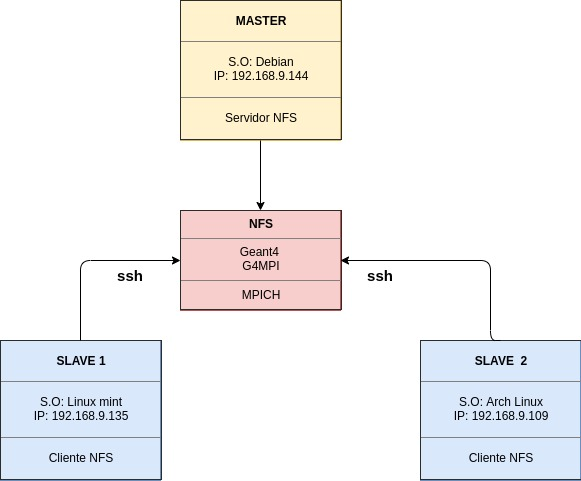
\includegraphics[width=0.7\textwidth]{images/EsquemaGeneral.jpg}
  \caption{Esquema}
  \label{esq}
\end{figure}


\newpage
\section{Instalación de Geant4}
\subsection{Instalación de prerrequisitos}

\begin{itemize}
    \item \textbf{CLHEP}
    \url{http://proj-clhep.web.cern.ch/proj-clhep/clhep23.html} \\
leer el archivo README.txt luego crear una carpeta Build y una install dentro de la carpeta build hacer:

\begin{lstlisting}[language=bash,style=mystyle]
cmake -DCMAKE_INSTALL_PREFIX=<install_dir> <source_code_dir>
cmake --build . --config RelWithDebInfo
cmake --build . --target install
\end{lstlisting} 




    \item \textbf{Zlib}%%%%%%%%%%%%%%%%%%%%%%%%%%%%%%%%%%%%
    
\begin{lstlisting}[language=bash,style=mystyle]
sudo apt install zlib1g-dev 
\end{lstlisting}     
    
    
    \item \textbf{QT}%%%%%%%%%%%%%%%%%%%%%%%%%%%%%%%%%%%%%%%%
    
\begin{lstlisting}[language=bash,style=mystyle]
sudo apt install qt4-default
\end{lstlisting}      
    
    
    \item \textbf{OpenGL}%%%%%%%%%%%%%%%%%%%%%%%%%%%%%%%%%%%%%
    
\begin{lstlisting}[language=bash,style=mystyle]
sudo apt-get install libglu1-mesa-dev freeglut3-dev mesa-common-dev
\end{lstlisting}      
    
    
    \item \textbf{ray tracer}%%%%%%%%%%%%%%%%%555
    
\begin{lstlisting}[language=bash,style=mystyle]
sudo apt install povray
\end{lstlisting}     
    
    
    \item \textbf{X11 libraries}%%%%%%%%%%%%%%%%%%%%%%%%%%%%%%%%%%%%
    
\begin{lstlisting}[language=bash,style=mystyle]
sudo apt-get install xorg-dev
\end{lstlisting}  


    \item \textbf{X11 libraries}%%%%%%%%%%%%%%%%%%%%%%%%%
    
\begin{lstlisting}[language=bash,style=mystyle]
sudo apt-get install xorg-dev
\end{lstlisting} 


    \item \textbf{g++ y gcc}%%%%%%%%%%%%%%%%%%%%%%%%%%%%%%%%%
    
\begin{lstlisting}[language=bash,style=mystyle]
sudo apt-get update -y && \

sudo apt-get install -y wget g++-5 gcc-5 cmake libexpat1-dev vim cmake-curses-gui freeglut3 freeglut3-dev mesa-utils python libx11-dev libxmu-dev expat && \

sudo apt-get install -y libfontconfig1-dev libfreetype6-dev libxcursor-dev libxext-dev libxfixes-dev libxft-dev libxi-dev libxrandr-dev libxrender-dev && \

sudo apt-get install libssl-dev
\end{lstlisting} 


\end{itemize}{}


\newpage

\subsection{Instalación de Geant4}

\begin{enumerate}
    \item Creación de carpetas donde estará alojada la instalación
    
\begin{lstlisting}[language=bash,style=mystyle]

$ cd $HOME
$ sudo mkdir -p $HOME/Geant4-10.6/src 
$ sudo mkdir -p $HOME/Geant4-10.6/build 
$ sudo mkdir -p $HOME/Geant4-10.6/install 
$ sudo mkdir -p $HOME/Geant4-10.6/data 

\end{lstlisting}
    
    \item Descarga de Geant4:
    
\begin{lstlisting}[language=bash,style=mystyle]

$ G4_VERSION="10.06.p01"
$ QT_VERSION="4.8.7"
$ sudo wget http://cern.ch/geant4-data/releases/geant4.${G4_VERSION}.tar.gz
$ sudo tar xf geant4.${G4_VERSION}.tar.gz -C $HOME/Geant4-10.6/src
$ sudo rm geant4.${G4_VERSION}.tar.gz 

\end{lstlisting}     


    \item Compilación:
    
\begin{lstlisting}[language=bash,style=mystyle]

$ cd $HOME/Geant4-10.6/build
$ cmake -DCMAKE_INSTALL_PREFIX=$HOME/Geant4-10.6/install \
      -DGEANT4_USE_OPENGL_X11=ON \
      -DQT_QMAKE_EXECUTABLE=/usr/local/Trolltech/Qt-${QT_VERSION}/bin/qmake \
      -DGEANT4_USE_QT=OFF \
      -DGEANT4_INSTALL_DATA=ON \
      -DGEANT4_INSTALL_DATADIR=$HOME/Geant4-10.6/data \
      -DGEANT4_BUILD_MULTITHREADED=ON \
      -DGEANT4_INSTALL_EXAMPLES=ON \
      ../src/geant4.${G4_VERSION}
      
$ make -j`nproc` 

\end{lstlisting}     

    
    \item Instalación:

\begin{lstlisting}[language=bash,style=mystyle]

$ sudo make install
 
\end{lstlisting}     

    \item Cargar varibles de entorno:

\begin{lstlisting}[language=bash,style=mystyle]

$ echo "export LD_LIBRARY_PATH=${LD_LIBRARY_PATH}:/usr/local/Trolltech/Qt-${QT_VERSION}/lib" >> $HOME/.bashrc
$ echo "source $HOME/Geant4-10.6/install/bin/geant4.sh" >> $HOME/.bashrc


\end{lstlisting}     


    \item Verificar instalación y configuración


\begin{lstlisting}[language=bash,style=mystyle]

$ ./geant4-config --help
 
\end{lstlisting} 

\item Por último crear variables de entorno:


\begin{lstlisting}[language=bash,style=mystyle]
echo "source $HOME/geant4/install/bin/geant4.sh" >> $HOME/.bashrc
\end{lstlisting} 

\end{enumerate}

\newpage

\subsubsection{Configurar variables de entorno para Geant4}

\begin{enumerate}
    \item Abrir el archivo bashrc:
    
\begin{lstlisting}[language=bash,style=mystyle]

$ sudo nano ~/.bashrc

\end{lstlisting} 

    \item Añadir al final las siguiente líneas:
    
\begin{lstlisting}[language=bash,style=mystyle]

export G4ABLADATA=/home/gfnun/Geant4-10.6/install/share/Geant4-10.6.1/data/G4ABLA3.1
export G4ENSDFSTATEDATA=/home/gfnun/Geant4-10.6/install/share/Geant4-10.6.1/data/G4ENSDFSTATE2.2
export G4INCLDATA=/home/gfnun/Geant4-10.6/install/share/Geant4-10.6.1/data/G4INCL1.0
export G4LEDATA=/home/gfnun/Geant4-10.6/install/share/Geant4-10.6.1/data/G4EMLOW7.9.1
export G4LEVELGAMMADATA=/home/gfnun/Geant4-10.6/install/share/Geant4-10.6.1/data/PhotonEvaporation5.5
export G4NEUTRONHPDATA=/home/gfnun/Geant4-10.6/install/share/Geant4-10.6.1/data/G4NDL4.6
export G4PARTICLEXSDATA=/home/gfnun/Geant4-10.6/install/share/Geant4-10.6.1/data/G4PARTICLEXS2.1
export G4PIIDATA=/home/gfnun/Geant4-10.6/install/share/Geant4-10.6.1/data/G4PII1.3
export G4REALSURFACEDATA=/home/gfnun/Geant4-10.6/install/share/Geant4-10.6.1/data/RealSurface2.1.1
export G4SAIDXSDATA=/home/gfnun/Geant4-10.6/install/share/Geant4-10.6.1/data/G4SAIDDATA2.0

\end{lstlisting}
\end{enumerate}


\subsubsection{Ejecutar Ejemplo B1}

\begin{enumerate}

    \item Ir a la carpeta del código fuente del ejemplo y crear una carpeta para la compilación.
    
\begin{lstlisting}[language=bash,style=mystyle]

$ cd /home/gfnun/Geant4-10.6/src/geant4.10.06.p01/examples/basic/B1
$ mkdir build-B1 

\end{lstlisting}

    \item Compilar y ejecutar:
    
\begin{lstlisting}[language=bash,style=mystyle]

$ cmake –DGeant4_DIR=/home/gfnun/Geant4-10.6/install/lib/Geant4-10.6.1 /home/gfnun/Geant4-10.6/src/geant4.10.06.p01/examples/basic/B1
$ make -j4
$ ./exampleB1

\end{lstlisting}  

\end{enumerate}

\newpage










    
    

%\section{Herramientas para la computación distribuida}
%Aquí meter la teoría de MPI/ G4 mpi / lo que encontrol de LAM y demás...etc
\begin{figure}[H]
    \centering
  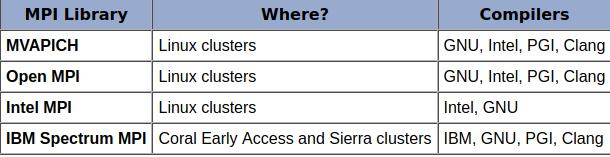
\includegraphics[width=0.7\textwidth]{images/compil.jpg}
  \caption{Implementaciones}
  \label{acce}
\end{figure}


\begin{figure}[H]
    \centering
  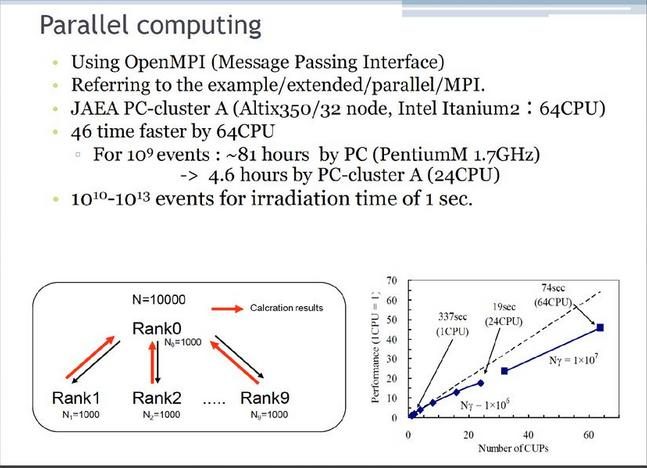
\includegraphics[width=0.7\textwidth]{images/paper.jpg}
  \caption{Paper}
  \label{acce}
\end{figure}

\newpage
%\section{Laboratorio de pruebas}
Describir el laboratorio de Pruebas

\begin{figure}[H]
    \centering
  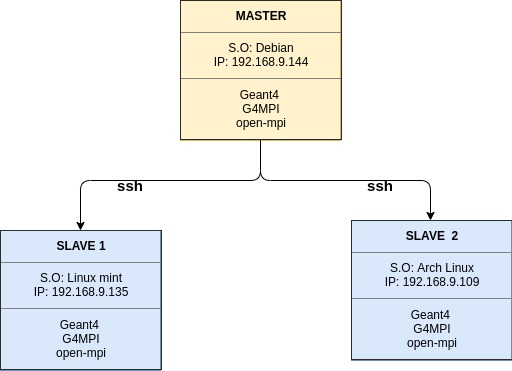
\includegraphics[width=0.7\textwidth]{images/esquema.jpg}
  \caption{Esquema}
  \label{esq}
\end{figure}


\begin{figure}[H]
    \centering
  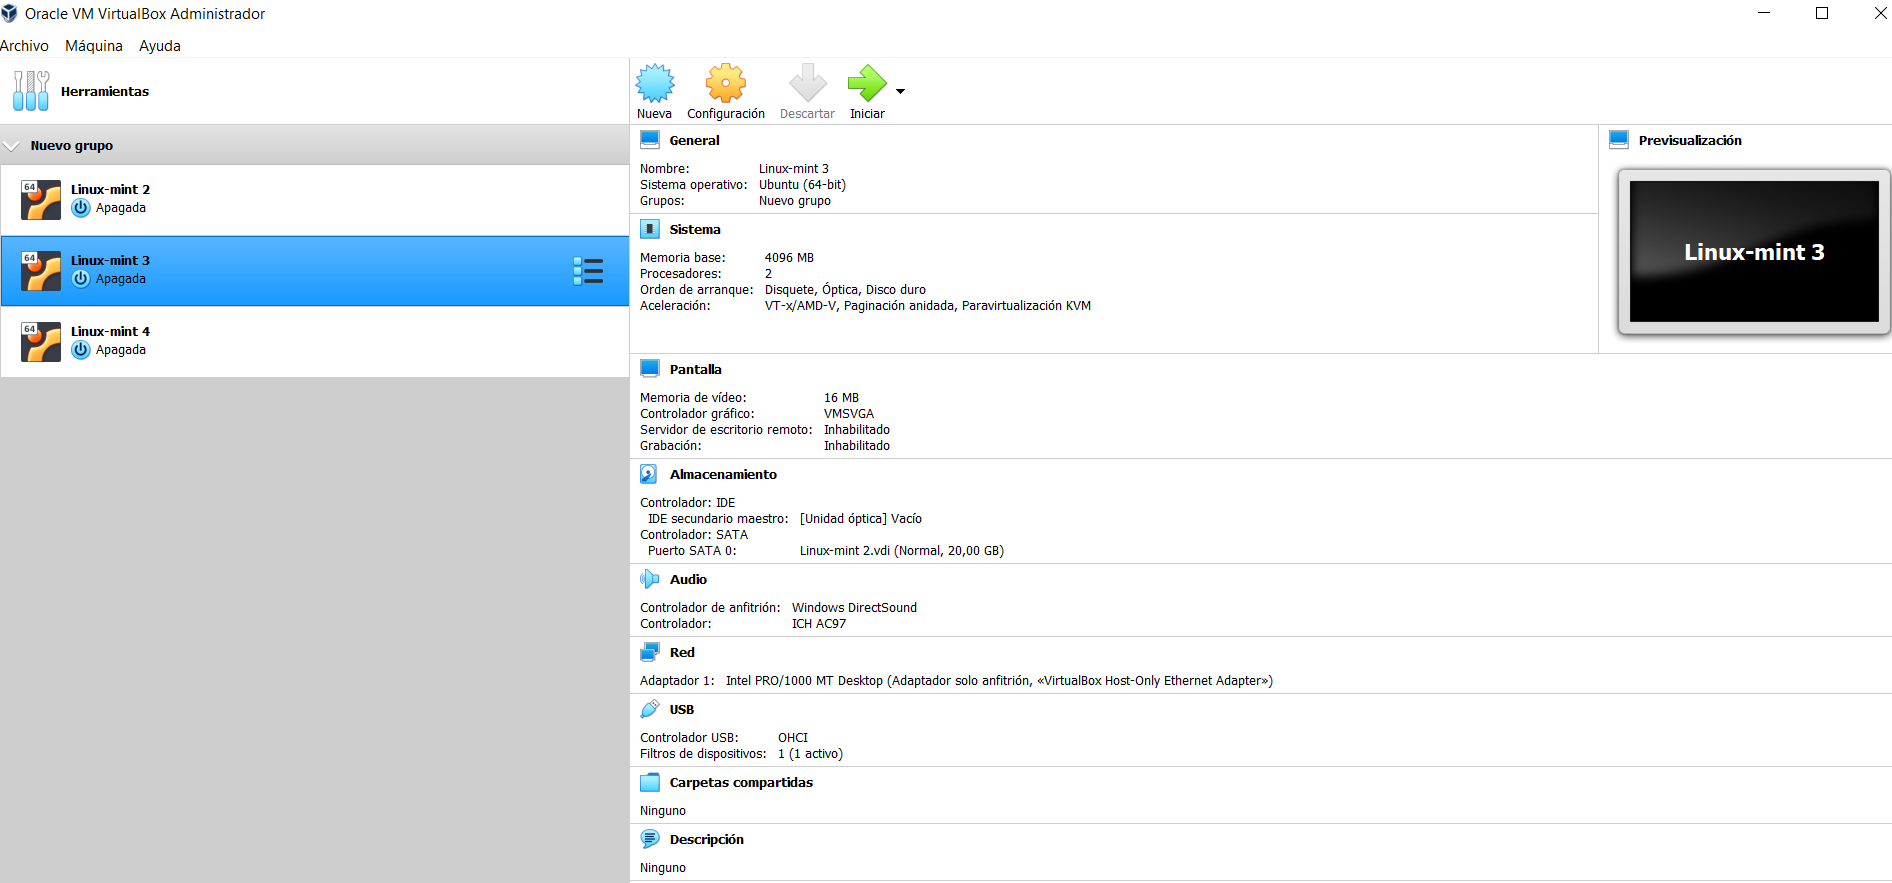
\includegraphics[width=0.7\textwidth]{images/lab1.PNG}
  \caption{Máquina Virtual}
  \label{mv1}
\end{figure}


\begin{figure}[H]
    \centering
  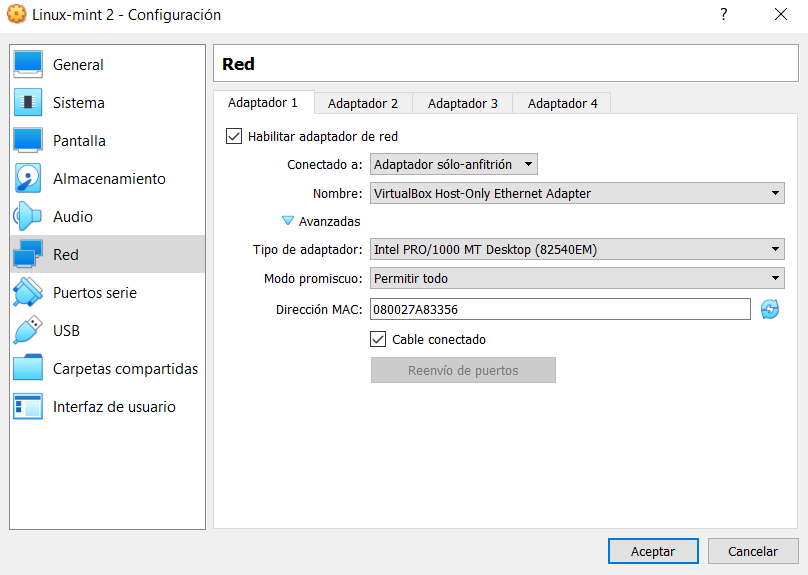
\includegraphics[width=0.7\textwidth]{images/lab2.PNG}
  \caption{Máquina Virtual}
  \label{mv2}
\end{figure}

\begin{figure}[H]
    \centering
  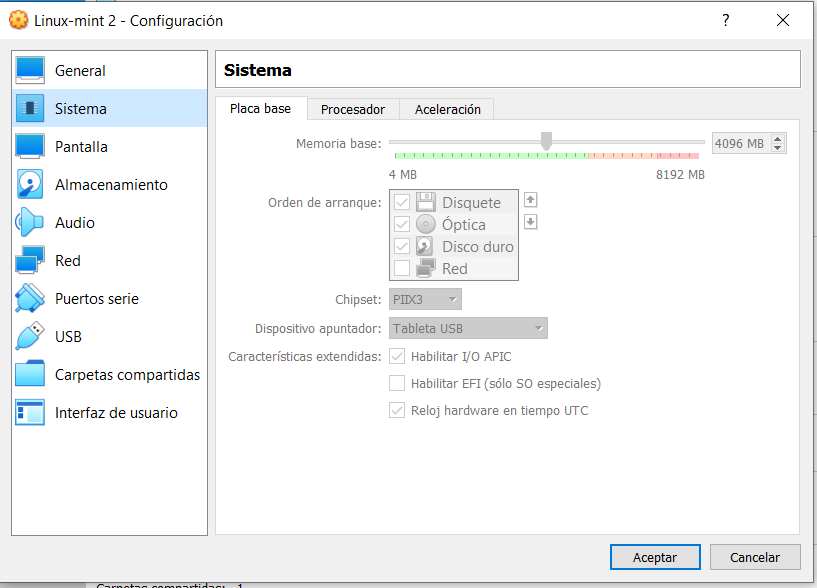
\includegraphics[width=0.7\textwidth]{images/lab3.PNG}
  \caption{Máquina Virtual}
  \label{mv3}
\end{figure}


\begin{figure}[H]
    \centering
  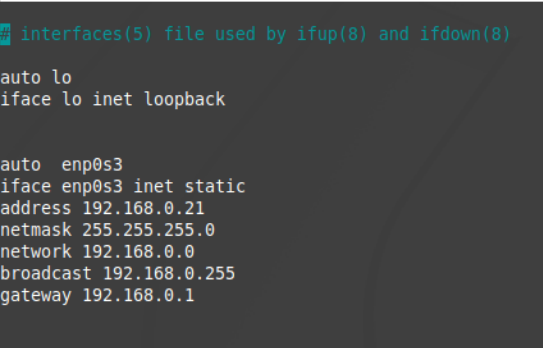
\includegraphics[width=0.7\textwidth]{images/lab4.PNG}
  \caption{ip estática}
  \label{mv4}
\end{figure}


\begin{figure}[H]
    \centering
  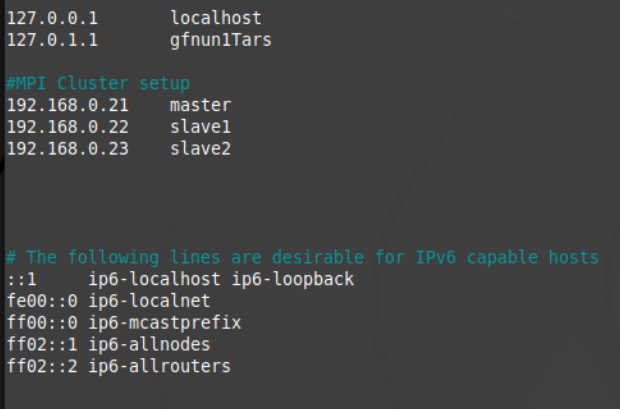
\includegraphics[width=0.7\textwidth]{images/lab5.PNG}
  \caption{Archivo hosts}
  \label{mv5}
\end{figure}



\newpage
\section{Configuraciones básicas de cada equipo}

\subsection{Configuración de usuarios de cada máquina}
Todas las máquinas se configuran con el mismo nombre de usuario, así en cada máquina
abrimos una terminal y ejecutamos los siguientes comandos:

\begin{enumerate}
    \item Entrar al modo root:
    
\begin{lstlisting}[language=bash, style=mystyle]
$ ifconfig -a
\end{lstlisting} 


    \item Agregar el usuario:
    
\begin{lstlisting}[language=bash, style=mystyle]
$ adduser gfnun
\end{lstlisting} 

Se solicitara el ingreso de la clave y unos datos adicionales los cuales deberan
ingresarse si se desea, de lo contrario solo hacer \textit{enter} y continuar.
    

    \item Comprobar que se creo el usuario:
    
\begin{lstlisting}[language=bash, style=mystyle]
$ cd ~
$ ls /home
\end{lstlisting}

    \item Se debera ver la carpeta del usuario, adicional ingresamos para comprobar:
    
\begin{lstlisting}[language=bash, style=mystyle]
$ ssh gfnun@0.0.0.0
\end{lstlisting}

    \item Salir y se le da permisos de administrador, desde el root:
    
\begin{lstlisting}[language=bash, style=mystyle]
$ exit
$ adduser gfnun sudo
\end{lstlisting}
    
\end{enumerate}



\subsection{Configurar ip estática}

\begin{enumerate}
    
    \item Comprobar las interfaces de red que tiene el equipo.
    
\begin{lstlisting}[language=bash,style=mystyle]
$ ifconfig -a
\end{lstlisting}


    \item Edita el archivo de configuración de las interfaces de red con el siguiente comando:
    
\begin{lstlisting}[]
sudo nano /etc/network/interfaces
\end{lstlisting} 

    \item En este caso se va configurar la interfaz eth0,
    
\begin{lstlisting}[language=bash, style=mystyle]
# Configuración de dirección IP fija para el interfaz eth0
auto eth0
iface eth0 inet static
address 192.168.1.50
netmask 255.255.255.0
network 192.168.1.0
broadcast 192.168.1.255
gateway 192.168.1.1
\end{lstlisting} 


    \item Reiniciar las interfaces de red del equipo:
    
\begin{lstlisting}[language=bash,style=mystyle]
$ sudo /etc/init.d/networking restart
\end{lstlisting} 


    \item Alternativamente:
    
\begin{lstlisting}[language=bash,style=mystyle]
$ sudo ifconfig eth0 down 
$ sudo ifconfig eth0 up
\end{lstlisting} 

\end{enumerate}



\subsection{Configurar archivo \emph{Hosts}}

Configurar el archivo hosts con las ip de los PC's con los que se va hacer el \emph{cluśter} (ver sección configuraciones básicas de cada equipo, para configuración de ip estática). 

Para ingresar al archivo:

\begin{lstlisting}[language=bash,style=mystyle2]
$ sudo nano /etc/hosts
\end{lstlisting} 

El archivo \emph{hosts} debe quedar así. En este caso tenemos dos esclavos y un maestro.

\begin{lstlisting}[language=bash,caption={Archivo hosts en el maestro},style=mystyle2]
127.0.0.1       localhost
127.0.1.1       MrHerbert.gfnun.unal.edu.co     MrHerbert

#MPI Cluster Setup
192.168.9.144 master
192.168.9.135 slave1
192.168.9.109 slave2

# The following lines are desirable for IPv6 capable hosts
::1     localhost ip6-localhost ip6-loopback
ff02::1 ip6-allnodes
ff02::2 ip6-allrouters

\end{lstlisting} 


También se debe configurar el de cada esclavo así:

\begin{lstlisting}[language=bash,caption={Archivo hosts esclavo 1},style=mystyle2]
#MPI Cluster Setup
192.168.9.144 master
192.168.9.109 slave1

# The following lines are desirable for IPv6 capable hosts
::1     localhost ip6-localhost ip6-loopback
ff02::1 ip6-allnodes
ff02::2 ip6-allrouters

\end{lstlisting} 

Para el esclavo 2:

\begin{lstlisting}[language=bash,caption={Archivo esclavo 1},style=mystyle2]
#MPI Cluster Setup
192.168.9.144 master
192.168.9.109 slave2

# The following lines are desirable for IPv6 capable hosts
::1     localhost ip6-localhost ip6-loopback
ff02::1 ip6-allnodes
ff02::2 ip6-allrouters

\end{lstlisting} 



\subsection{Configurar ssh}
Lo siguiente es configurar los accesos a través de ssh entre las máquinas para que no
solicite clave cada vez que la máquina maestro (master) acceda a cada esclavo (slave1, slave2..etc)

\begin{enumerate}
    \item En el Master, generar la llave rsa:
    
\begin{lstlisting}[language=bash,style=mystyle]
$ ssh-keygen -t rsa
\end{lstlisting} 

    \item Verificar si se tiene el archivo authorized\_keys, hacer esto para cada nodo:
    
\begin{lstlisting}[language=bash,style=mystyle]
$ ls -l .ssh/
\end{lstlisting}

    \item Si no se encuentra, crearlo:
\begin{lstlisting}[language=bash,style=mystyle]
$ touch ~/.ssh/authorized_keys
\end{lstlisting} 

    \item Generar permisos al archivo:
\begin{lstlisting}[language=bash,style=mystyle]
$ chmod 600 ~/.ssh/authorized_keys
\end{lstlisting}

    \item Copiar llaves generadas desde el master a los esclavos:
\begin{lstlisting}[language=bash,style=mystyle]
$ scp .ssh/id_rsa.pub gfnun@slave1:.ssh/authorized_keys
$ scp .ssh/id_rsa.pub gfnun@slave2:.ssh/authorized_keys
\end{lstlisting}

    \item También se debe copiar en el mismo master para que no solicite clave al hacer ssh sobre el mismo:
\begin{lstlisting}[language=bash,style=mystyle]
$ cp ~/.ssh/id_rsa.pub ~/.ssh/authorized_keys
\end{lstlisting}

    \item Para el esclavo dos
\begin{lstlisting}[language=bash,style=mystyle]
$ scp .ssh/id_rsa.pub gfnun@slave2:.ssh/authorized_keys
\end{lstlisting} 

Esto es importante ya que con la implementación de mpi a veces se desea usar el mismo master para ejecutar aplicaciones.

    \item Así no pedirá contraseña cada vez que se va ingresar a cada nodo desde el master, bastara escribir algo así:
    
\begin{lstlisting}[language=bash,style=mystyle]
$ ssh slave2
\end{lstlisting} 
    
\end{enumerate}






 















\newpage


\section{Instalación y configuración de servidor NFS}


NFS (sistema de archivos de red: «Network File System») es un protocolo que permite acceso remoto a un sistema de archivos a través de la red. Todos los sistemas Unix pueden trabajar con este protocolo.

% Para el montaje de este servidor en las máquinas con debian y arch linux se basa en la siguiente información

% \begin{itemize}
%     \item \url{http://l.github.io/debian-handbook/html/es-ES/sect.nfs-file-server.html}
    
%     \item \url{https://wiki.archlinux.org/index.php/NFS}      
    
    
% \end{itemize}

\subsection{Configuración servidor}

\begin{enumerate}

    \item En el master
    
\begin{lstlisting}[language=bash,style=mystyle] 
$ sudo apt install nfs-kernel-server portmap
$ mkdir sharedFolder
$ ls sharedFolder/ 
\end{lstlisting}

    \item Cambiar el propietario de la carpeta a nadie.
    
\begin{lstlisting}[language=bash,style=mystyle]    
$ sudo chown nobody:nogroup sharedFolder/
\end{lstlisting} 


    \item Ver el estado del servidor:
    
\begin{lstlisting}[language=bash,style=mystyle]    
$ sudo /etc/init.d/nfs-kernel-server status
\end{lstlisting} 


    \item Detener el servicio:
    
\begin{lstlisting}[language=bash,style=mystyle]    
$ sudo /etc/init.d/nfs-kernel-server stop
\end{lstlisting} 


    \item Modificar el archivo exports:
    
\begin{lstlisting}[language=bash,style=mystyle]    
$ sudo pico /etc/exports
\end{lstlisting} 


    \item Añadir:
    
\begin{lstlisting}[language=bash,style=mystyle]    
/home/gfnun/sharedFolder/ *(rw,sync,no_subtree_check)
/home/gfnun/Geant4-10.6/ *(rw,sync,no_subtree_check)
/home/gfnun/Geant4-10.5/ *(rw,sync,no_subtree_check)
\end{lstlisting} 



    \item Volver a la terminal, y hacer que todos los directorios colocados allí se exporten:
    
\begin{lstlisting}[language=bash,style=mystyle]    
$ sudo exportfs -a
\end{lstlisting} 


    \item Verificar:
    
\begin{lstlisting}[language=bash,style=mystyle]    
$ sudo exportfs
\end{lstlisting} 


    \item Salida en la terminal:
    
\begin{lstlisting}[language=bash,style=mystyle]    
/home/gfnun/sharedFolder
		<world>
/home/gfnun/Geant4-10.6
		<world>
/home/gfnun/Geant4-10.5
		<world>
\end{lstlisting} 


    \item En los esclavos:
    
\begin{lstlisting}[language=bash,style=mystyle]    
$ sudo apt-get install nfs-common portmap
$ mkdir -p sharedFolder/
$ ls sharedFolder
$ mkdir -p Geant4-10.6/
$ ls sharedFolder
\end{lstlisting} 


    \item En el maestro iniciar el servidor:
    
\begin{lstlisting}[language=bash,style=mystyle]    
$ sudo /etc/init.d/nfs-kernel-server start
\end{lstlisting} 


    \item Ver el estado:
    
\begin{lstlisting}[language=bash,style=mystyle]    
$ sudo /etc/init.d/nfs-kernel-server status
\end{lstlisting} 

    \item Ahora compartir las carpetas en cada esclavo, por ejemplo para el esclavo 1 (\emph{slave1}):
    
\begin{lstlisting}[language=bash,style=mystyle] 
$ ssh slave1
$ sudo mount master:/home/gfnun/sharedFolder sharedFolder/
$ sudo mount master:/home/gfnun/Geant4-10.6/ Geant4-10.6/
$ sudo mount master:/home/gfnun/Geant4-10.5/ Geant4-10.5/
\end{lstlisting} 


    \item Verificar que se esta compartiendo:
    
\begin{lstlisting}[language=bash,style=mystyle]    
$ df -h
\end{lstlisting}


    \item La salida debería ser:
    
\begin{lstlisting}[language=bash,style=mystyle]    
master:/home/gfnun/sharedFolder               723G  440G  247G  65% /home/gfnun/sharedFolder
master:/home/gfnun/Geant4-10.6                723G  440G  247G  65% /home/gfnun/Geant4-10.6
master:/home/gfnun/Geant4-10.6                723G  440G  247G  65% /home/gfnun/Geant4-10.5
\end{lstlisting} 


    \item En uno de los esclavos podemos probar que se comparten los archivos:
    
\begin{lstlisting}[language=bash,style=mystyle]    
$ cd sharedFolder/
$ touch test.txt
\end{lstlisting} 

y verificar que se vea desde el maestro.


\end{enumerate}



\newpage
%\section{Instalación y configuración de MPICH}

\subsection{Instalando MPICH2}

\begin{itemize}


    \item Descargar MPICH \url{http://www.mpich.org/downloads/}
    

    \item Descomprimir
\begin{lstlisting}[language=bash,style=mystyle]     
tar -xzf mpich-3.3.2.tar.gz 
\end{lstlisting}   

    \item Compilar e instalar 
\begin{lstlisting}[language=bash,style=mystyle]    
cd mpich-3.3.2
sudo mkdir build
cd build
sudo mkdir ../mpich-install
  
sudo ../configure --prefix=/home/gfnun/mpich-install/ --disable-fc --disable-f77 --enable-shared
\end{lstlisting} 


\item Aparece el siguiente error:

\begin{lstlisting}[language=bash,style=mystyle2]  
configure: error: No Fortran 77 compiler found. If you dont need to build any Fortran programs, you can disable Fortran support using --disable-fortran. If you do want to build Fortran programs, you need to install a Fortran compiler such as gfortran or ifort before you can proceed.
\end{lstlisting} 



\item Corrección error, debido a que no está instalado Fortran, para este caso no se necesita, por ende se coloca la bandera de desactivación.

\begin{lstlisting}[language=bash,style=mystyle]    
sudo ../configure --prefix=/home/gfnun/mpich-install/ --disable-fc --disable-f77 --enable-shared --disable-fortran 
\end{lstlisting} 



\item Aparece el mensaje:

\begin{lstlisting}[language=bash,style=mystyle2]    
Configuration completed.
\end{lstlisting} 



\item Compilación e instalación.

\begin{lstlisting}[language=bash,style=mystyle]      
sudo make
sudo make install
\end{lstlisting} 


\item Hacer la siguiente exportación de las variables de entorno con las que se va a trabajar.

\begin{lstlisting}[language=bash,style=mystyle]     
export PATH=/home/gfnun/sharedFolder/mpich-install/bin:$PATH
export LD_LIBRARY_PATH=/home/gfnun/sharedFolder/mpich-install/lib:$LD_LIBRARY_PATH 
\end{lstlisting} 



\end{itemize}
\section{Instalación de Open-MPI}

Descargar open-mpi desde \url{https://www.open-mpi.org/software/ompi/v4.0/}, se descarga el archivo openmpi-4.0.3.tar.gz. Dejarlo en el directorio:

\begin{lstlisting}[language=bash,style=mystyle]    
$ pwd
/home/gfnun/
\end{lstlisting} 


\begin{enumerate}

    \item Descomprimir en la carpeta sharedFolder/ :
\begin{lstlisting}[language=bash,style=mystyle]    
$ cp openmpi-4.0.3.tar.gz sharedFolder/
$ cd sharedFolder/
$ mkdir openmpi-install/
$ tar -xzf openmpi-4.0.3.tar.gz   
\end{lstlisting}
 
    \item Compilar:
\begin{lstlisting}[language=bash,style=mystyle]  
$ cd openmpi-4.0.3/
$ mkdir build
$ cd build
$ ../configure --prefix=/home/gfnun/sharedFolder/openmpi-install/ --enable-mpi-cxx --enable-orterun-prefix-by-default 
$ sudo make -j4      
\end{lstlisting}
    
    \item Instalar:
\begin{lstlisting}[language=bash,style=mystyle] 
$ sudo make install
$ sudo ldconfig      
\end{lstlisting}
    
    \item Para usar open mpi instalado en la carpeta sharedFolder/ cargamos las variables de entorno:
\begin{lstlisting}[language=bash,style=mystyle]
$ export PATH=/home/gfnun/sharedFolder/openmpi-install/bin:$PATH
$ export LD_LIBRARY_PATH=/home/gfnun/sharedFolder/openmpi-install/lib:$LD_LIBRARY_PATH
\end{lstlisting}   
    
    \item Si se desea, se puede dejar en el bashrc:
\begin{lstlisting}[language=bash,style=mystyle]
echo "export PATH=/home/gfnun/sharedFolder/openmpi-install/bin:$PATH" >> $HOME/.bashrc
echo "export LD_LIBRARY_PATH=/home/gfnun/sharedFolder/openmpi-install/lib:$LD_LIBRARY_PATH" >> $HOME/.bashrc
\end{lstlisting}

así cargara automáticamente las variables de entorono de mpi cada vez que se inicie sesión.
    
\end{enumerate}



\subsection{Configurar Cluster}

Crear un archivo en donde vamos a listar los nodos del \emph{clúster} (nodos se refiere a cada máquina del \emph{clúster}). En este archivo se indica los procesos a usar por máquina. 

A continuación se presentan ejemplos del archivo: 

\begin{itemize}
    \item Creación del Archivo:
\begin{lstlisting}[language=bash,style=mystyle]
sudo touch my_hosts 
\end{lstlisting}


    \item Añadir las siguientes líneas, indicando el número de hilos a usar por cada nodo:
    
\begin{lstlisting}[language=bash,style=mystyle2]
master slots=1
slave1 slots=2
slave2 slots=2
\end{lstlisting}

    \item Ejecutar ejemplo:
\begin{lstlisting}[language=bash,style=mystyle2]
$ cd ..
$ cd examples
$ sudo mpicc hello_c.c -o hello_c
$ mpiexec -np 4 --hostfile my_hosts ./hello_cslave1
slave2
\end{lstlisting}

\end{itemize}



\subsection{Ejemplo de Comandos MPI}


\begin{lstlisting}[language=bash,style=mystyle2]
mpirun -np 6 --hostfile my_hosts openmpi-4.0.3/examples/hello_c | sort
mpirun -H slave1,slave2 openmpi-4.0.3/examples/hello_c | sort
mpirun -H master,slave1,slave2 openmpi-4.0.3/examples/hello_c | sort
mpirun -H master,slave1,slave2,slave2 openmpi-4.0.3/examples/hello_c | sort
mpirun -H master,slave1,slave2 -npernode 2 openmpi-4.0.3/examples/hello_c | sort
\end{lstlisting} 


\newpage
\section{Compilar G4mpi}

G4MPI es una interfaz nativa con bibliotecas MPI. El directorio contiene una biblioteca de IU de Geant4 y un par de ejemplos paralelizados. Con esta interfaz, las aplicaciones de los usuarios se pueden paralelizar con diferentes bibliotecas compatibles con MPI, como OpenMPI, LAM / MPI, MPICH2, etc.

\begin{figure}[H]
    \centering
  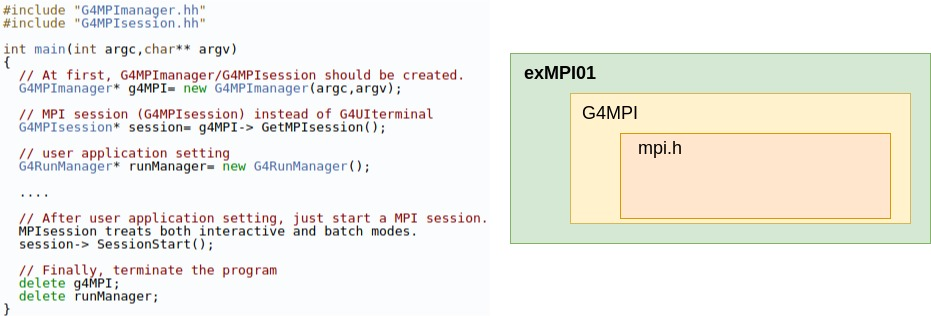
\includegraphics[width=0.7\textwidth]{images/estructure.jpg}
  \caption{Esquema}
  \label{esq}
\end{figure}

\subsection{Compilando G4mpi}


\begin{lstlisting}[language=bash,style=mystyle]   
mkdir build-mpi
cd build-mpi
cmake -DGeant4_DIR=/home/gfnun1/geant4/install/lib/Geant4-10.6.1 \
     -DCMAKE_INSTALL_PREFIX=/home/gfnun1/geant4/geant4-mpi \
     /home/gfnun1/geant4/src/geant4.10.06.p01/examples/extended/parallel/MPI/source
make
make install  
\end{lstlisting}


\subsection{Compilando Ejemplo exMP01}

\begin{lstlisting}[language=bash,style=mystyle]   
mkdir build
cd build
cmake -DG4mpi_DIR=<where-G4mpi-wasintalled>/lib[64]/G4mpi -DCMAKE_CXX_COMPILER=mpicxx \
      -DGeant4_DIR=<your Geant4 install path>/lib[64]/Geant4-V.m.n <path-to-source>
      (V.m.n is the version of Geant4, eg. Geant4-9.6.0)
make
make install
\end{lstlisting}

\begin{lstlisting}[language=bash,style=mystyle]
mkdir build
cd build
sudo cmake -DG4mpi_DIR=/home/gfnun/geant4/geant4-mpi/lib/G4mpi-10.6.1 -DCMAKE_CXX_COMPILER=mpicxx \
      -DGeant4_DIR=/home/gfnun/geant4/install/lib/Geant4-10.6.1 /home/gfnun1/geant4/src/geant4.10.06.p01/examples/extended/parallel/MPI/examples/exMPI01
make
make install 
\end{lstlisting}

\subsection{Ejecutando Ejemplo con open-mpi}

\begin{lstlisting}[language=bash,style=mystyle]
$ mpirun -np 3 --hostfile /home/gfnun1/my_hosts ./exMPI01
\end{lstlisting}

\newpage



\section{Ejecutando ejemplos de geant4 en el sistema distribuido}

\subsection{Ejemplo exMPI01}

En esta sección se va ejecutar el ejemplo exMP01, ubicado en:

\begin{lstlisting}[language=bash,style=mystyle]
cd /home/gfnun/geant4.10.06/src/geant4.10.06.p01/examples/extended/parallel/MPI/examples/exMPI01
\end{lstlisting}

La documentación nos indica como debemos compilar el ejemplo.
\begin{lstlisting}[language=bash,style=mystyle]
mkdir build
cd build
cmake -DG4mpi_DIR=<where-G4mpi-wasintalled>/lib[64]/G4mpi -DCMAKE_CXX_COMPILER=mpicxx \
      -DGeant4_DIR=<your Geant4 install path>/lib[64]/Geant4-V.m.n <path-to-source>
      (V.m.n is the version of Geant4, eg. Geant4-9.6.0)
make
make install
\end{lstlisting}

Para este caso el ejemplo se compila así:

\begin{lstlisting}[language=bash,style=mystyle]
$ mkdir build
$ cd build
$ sudo cmake -DG4mpi_DIR=/home/gfnun/Geant4-10.6/geant4-mpi/lib/G4mpi-10.6.1 -DCMAKE_CXX_COMPILER=mpicxx \
      -DGeant4_DIR=/home/gfnun/Geant4-10.6/install/lib/Geant4-10.6.1 /home/gfnun/Geant4-10.6/src/geant4.10.06.p01/examples/extended/parallel/MPI/examples/exMPI01
$ sudo make
$ sudo make install
\end{lstlisting}

Ejecutar:

\begin{lstlisting}[language=bash,style=mystyle]
$ cd build
$ mpiexec -np 4 ./exMPI01
\end{lstlisting}

\subsection{Ejemplo exMPI04}

Compilar, para compilar se debe hacer desde el compilador de open mpi instalado en la carpeta sharedFolder/

\begin{lstlisting}[language=bash,style=mystyle]
$ mkdir build
$ cd build
$ sudo cmake -DG4mpi_DIR=/home/gfnun/Geant4-10.6/geant4-mpi/lib/G4mpi-10.6.1 -DCMAKE_CXX_COMPILER=/home/gfnun/sharedFolder/openmpi-install/bin/mpicxx \
      -DGeant4_DIR=/home/gfnun/Geant4-10.6/install/lib/Geant4-10.6.1 /home/gfnun/Geant4-10.6/src/geant4.10.06.p01/examples/extended/parallel/MPI/examples/exMPI04
$ make
$ make install
\end{lstlisting}

Ejecutar con Open mpi:

Exportar variables, en este caso la instalación de open mpi se realizó en sharedFolder:

\begin{lstlisting}[language=bash,style=mystyle]
export PATH=/home/gfnun/sharedFolder/openmpi-install/bin:$PATH
export LD_LIBRARY_PATH=/home/gfnun/sharedFolder/openmpi-install/lib:$LD_LIBRARY_PATH 
\end{lstlisting}

De esta manera se ejecuta en la máquina local:

\begin{lstlisting}[language=bash,style=mystyle]
$ cd build
$ mpiexec -n 4 ./exMPI04
\end{lstlisting}




% \begin{itemize}

%     \item \textbf{Usando MPICH:}
    
% Nos aseguramos de usar MPICH

% \begin{lstlisting}[language=bash,style=mystyle]     
% export PATH=/home/gfnun/sharedFolder/mpich-install/bin:$PATH
% export LD_LIBRARY_PATH=/home/gfnun/sharedFolder/mpich-install/lib:$LD_LIBRARY_PATH 
% \end{lstlisting}     

% Verificamos:

% \begin{lstlisting}[language=bash,style=mystyle]     
% which mpiexec
% \end{lstlisting} 

% Y debe arrojarnos el directorio desde donde se está ejecutando esta instrucción en este caso el directorio donde esta instalado MPICH.
% \\
% Creamos el archivo en dónde especificamos como usar los procesadores. Lo llamaremos \textbf{hostfile}, aquí le indicamos usar 1 procesador en el master, 4 para el escalvo 1 y 5 para el esclavo2.

% \begin{lstlisting}[language=bash,style=mystyle]     
% master:1
% slave1:4
% slave2:5
% \end{lstlisting}  

% En consola ejecutamos el siguiente comando:
% \begin{lstlisting}[language=bash,style=mystyle]     
% mpirun -f hostfile -n 10 ./exMPI01
% \end{lstlisting} 

% Si se desea especificar:
% \begin{lstlisting}[language=bash,style=mystyle]     
% mpirun -hosts slave1,slave2^Cn 2 ./exMPI01
% \end{lstlisting} 



%     \item \textbf{Usando open-MPI:}
    
% Creamos el archivo en dónde especificamos como usar los procesadores. Lo llamaremos \textbf{hostfile}, aquí le indicamos usar 1 procesador en el master, 4 para el escalvo 1 y 5 para el esclavo2.

% \begin{lstlisting}[language=bash,style=mystyle]     
% master slots=1
% slave1 slots=2
% slave2 slots=2
% \end{lstlisting}     
    
% \end{itemize}

\newpage






\section{Configurar una aplicación para uso con MPI}

Para este ejemplo se va usar la aplicación g4pntest, ubicada en este repositorio en la carpeta 00_g4_apps/

\subsection{Configuración sesión con G4mpi}

\begin{enumerate}
    \item Agregar las librerias necesarias para el uso de G4mpi, en PNtest.cc:

\begin{lstlisting}[language=bash,style=mystyle]
#include "G4MPImanager.hh"
#include "G4MPIsession.hh"
\end{lstlisting}
    
    \item Luego en la función main() del archivo PNtest.cc se añade las siguientes líneas de código, para este ejemplo se añade después de definir la semilla:

\begin{lstlisting}[language=bash,style=mystyle]
  // --------------------------------------------------------------------
  // MPI session
  // --------------------------------------------------------------------
  G4MPImanager* g4MPI = new G4MPImanager(argc, argv);
  // MPI session (G4MPIsession) instead of G4UIterminal
  // Terminal availability depends on your MPI implementation.
  G4MPIsession* session = g4MPI-> GetMPIsession();
  G4String prompt = "";
  prompt += "G4MPI";
  prompt += "(%s)[%/]:";
  session-> SetPrompt(prompt);
\end{lstlisting}
    
    \item En este caso la aplicación tiene activado Multithreading (MT), se debe dejar sin MT:
\begin{lstlisting}[language=bash,style=mystyle]
//#ifdef G4MULTITHREADED //Modified vy Javier
//  G4MTRunManager* runManager = new G4MTRunManager;
//  runManager-> SetNumberOfThreads(4);
//#else
  G4RunManager* runManager = new G4RunManager;
//#endif
\end{lstlisting}    
    
    \item Para la sesión se comentan o se quitan las siguientes líneas de código:
\begin{lstlisting}[language=bash,style=mystyle]
/* ORIGINAL
  // get the pointer to the User Interface manager
  G4UImanager* UI = G4UImanager::GetUIpointer();  

  if(argc == 1)
    {
#ifdef G4UI_USE
      G4UIExecutive* ui = new G4UIExecutive(argc, argv);
#ifdef G4VIS_USE
      UI->ApplyCommand("/control/execute vis.mac");
#endif
      ui->SessionStart();
      delete ui;
#endif
    }
  // Batch mode
  else
    {
      G4String command = "/control/execute ";
      G4String fileName = argv[1];
      UI->ApplyCommand(command+fileName);
    }
*/
\end{lstlisting}
    
    \item Se inicia la sesión:
\begin{lstlisting}[language=bash,style=mystyle]
session-> SessionStart();
\end{lstlisting}

    \item Por último se elimina la sesión de mpi agregando la siguiente línea de código antes del return 0:   
\begin{lstlisting}[language=bash,style=mystyle]
  delete g4MPI;
  delete runManager;
  return 0;
\end{lstlisting}    
\end{enumerate}



\subsection{Configuración CMakeLists.txt}


\begin{enumerate}

    \item Para el paquete de G4mpi agregar:
\begin{lstlisting}[language=bash,style=mystyle]
find_package(G4mpi REQUIRED) 
\end{lstlisting}

    \item Para incluir los directorios, se deja así:
\begin{lstlisting}[language=bash,style=mystyle]
include_directories(${CMAKE_CURRENT_SOURCE_DIR}/include
			      ${Geant4_INCLUDE_DIR}
			      ${G4mpi_INCLUDE_DIR})
\end{lstlisting}

    \item Añadir ejecutable y enlace con las librerias Geant4:
\begin{lstlisting}[language=bash,style=mystyle]
target_link_libraries(PNtest ${G4mpi_LIBRARIES})
\end{lstlisting}

\end{enumerate}



\subsection{Configuración archivos .csv}

\begin{enumerate}
    
    \item La función RunAction::BeginOfRunAction(const G4Run* aRun), se deja así, para la generación de cada archivo .csv en cada nodo o cada hilo:
\begin{lstlisting}[language=bash,style=mystyle]
void RunAction::BeginOfRunAction(const G4Run* aRun)
{
  G4cout << "### Run " << aRun->GetRunID() << " start." << G4endl;
  G4RunManager::GetRunManager()->SetRandomNumberStore(false);

  // ntuples will be written on each rank
  G4int rank = G4MPImanager::GetManager()->GetRank();
  std::ostringstream fname;
  fname<<"out_test-rank"<<rank;


  G4AnalysisManager* analysisManager = G4AnalysisManager::Instance();
  analysisManager->SetVerboseLevel(2);
  analysisManager->SetFileName(fname.str());

  analysisManager->OpenFile();
  analysisManager->CreateH1("Edep","Energy (keV)", 1000, 0., 1000.); // Id = 0
}
\end{lstlisting}


    \item Por último la función void RunAction::EndOfRunAction(const G4Run* aRun) se deja así:
    
\begin{lstlisting}[language=bash,style=mystyle]
void RunAction::EndOfRunAction(const G4Run* aRun)
{
  //if(!IsMaster()) return;
  //G4int nofEvents = aRun->GetNumberOfEvent();
  //if (nofEvents == 0) return;
  if(!IsMaster()) return;
  G4int nofEvents = aRun->GetNumberOfEvent();
  if (nofEvents == 0) return;

  G4cout << "RunActionMaster::EndOfRunAction" << G4endl;
  const G4int rank = G4MPImanager::GetManager()-> GetRank();
 
  G4cout << "=====================================================" << G4endl;
  G4cout << "Start EndOfRunAction for master thread in rank: " << rank<<G4endl;
  G4cout << "=====================================================" << G4endl;
 
  if ( !G4MPImanager::GetManager()->IsExtraWorker() ) {

    //Save histograms *before* MPI merging for rank #0
    if (rank == 0) {
      auto analysisManager = G4AnalysisManager::Instance();
      analysisManager->Write();
      analysisManager->CloseFile(false); // close without resetting histograms 
    }


      //Merge of g4analysis objects
      G4cout << "Go to merge histograms " << G4endl;
      G4MPIhistoMerger hm(G4AnalysisManager::Instance());
      hm.SetVerbosity(1);
      hm.Merge();
      G4cout << "Done merge histograms " << G4endl;
    }
 
   //Save g4analysis objects to a file
   //NB: It is important that the save is done *after* MPI-merging of histograms
   //One can save all ranks or just rank0, chane the if  
  if (true){  
  // if (rank == 0){
    auto analysisManager = G4AnalysisManager::Instance();
    if (rank == 0) {
      analysisManager->OpenFile("out_test-merged");  }
    analysisManager->Write();
    analysisManager->CloseFile();  }

   G4cout << "===================================================" << G4endl;
   G4cout << "End EndOfRunAction for master thread in rank: " << rank << G4endl;
   G4cout << "===================================================" << G4endl;


 // auto analysisManager = G4AnalysisManager::Instance();
 // analysisManager->Write();
 // analysisManager->CloseFile();
}
\end{lstlisting}



\end{enumerate}


\subsection{Configuración Clúster}

Para configurar el clúster y hacer uso de este con open mpi creamos un archio de texto plano llamado hostfile. Para este caso se tiene disponible 5 computadores con 8 hilos cada uno, es decir el clúster tiene 40 hilos disponibles. Si se desea usar todos los hilos disponibles el archivo debería erse así:

\begin{lstlisting}[language=bash,style=mystyle]
  master slots=8
  slave1 slots=8
  slave2 slots=8
  slave3 slots=8
  slave4 slots=8
\end{lstlisting}

Se puede administrar la cantidad de hilos a usar y en que computadores,por ejemplo:

\begin{lstlisting}[language=bash,style=mystyle]
  master slots=2
  slave1 slots=2
  slave2 slots=2
  slave3 slots=2
  slave4 slots=2
\end{lstlisting}

En este caso configuramos el \emph{clúster} para usar 2 hilos por cada computador lo que da un total de 10 hilos a usar por el \emph{clúster}.

\newpage

\subsection{Comando Ejecución con Open mpi}

A continuación el paso a paso para la ejecución de la aplicación:

Cargar variables de entorno:

\begin{lstlisting}[language=bash,style=mystyle]
$ source ~/Geant4-10.6/install/bin/geant4.sh
$ export PATH=/home/gfnun/sharedFolder/openmpi-install/bin:$PATH
$ export LD_LIBRARY_PATH=/home/gfnun/sharedFolder/openmpi-install/lib:$LD_LIBRARY_PATH
\end{lstlisting}


Compilar, para este caso por ejemplo el nombre de la carpeta donde se encuentra el proyecto es g4pntest_mpi:

\begin{lstlisting}[language=bash,style=mystyle]
$ cd g4pntest_mpi
$ mkdir build
$ cd build
$ cmake -DG4mpi_DIR=/home/gfnun/Geant4-10.6/geant4-mpi/lib/G4mpi-10.6.1 -DCMAKE_CXX_COMPILER=/home/gfnun/sharedFolder/openmpi-install/bin/mpicxx \
      –DGeant4_DIR=/home/gfnun/Geant4-10.6/install/lib/Geant4-10.6.1 ../
$ make -j`nproc`
\end{lstlisting}

Ejecución aplicación:

\begin{lstlisting}[language=bash,style=mystyle]
mpirun -np 40 -hostfile hostfile -x G4ABLADATA -x G4ENSDFSTATEDATA -x G4INCLDATA -x G4LEDATA -x G4LEVELGAMMADATA -x G4NEUTRONHPDATA -x G4PARTICLEXSDATA -x G4PIIDATA -x G4REALSURFACEDATA -x G4SAIDXSDATA -x G4RADIOACTIVEDATA -oversubscribe ./PNtest ../macros/THEmacro.mac
\end{lstlisting}

Si se requiere usar menos hilos, por ejemplo 12, el comando de ejecución sería así:

\begin{lstlisting}[language=bash,style=mystyle]
mpirun -np 12 -hostfile hostfile -x G4ABLADATA -x G4ENSDFSTATEDATA -x G4INCLDATA -x G4LEDATA -x G4LEVELGAMMADATA -x G4NEUTRONHPDATA -x G4PARTICLEXSDATA -x G4PIIDATA -x G4REALSURFACEDATA -x G4SAIDXSDATA -x G4RADIOACTIVEDATA -oversubscribe ./PNtest ../macros/THEmacro.mac
\end{lstlisting}


\newpage





\section{Rendimiento \emph{Clúster}}

\subsection{Variación número de hilos en el \emph{clúster}}

\begin{itemize}
    \item \textbf{Simulación:} G4pntest
    \item \textbf{Número de neutrones:} \num{10e6}
    \item \textbf{Energía:} 0.025 eV
    \item \textbf{Variación de Número de hilos con:} open MPI
    \item \textbf{Número de computadores:} 6
    \item \textbf{Número de hilos disponibles:} 48
    \item \textbf{Comando:} \$mpirun -np 3 -hostfile ./PNtest THEmacro.mac    
\end{itemize}

\begin{figure}[htb]
	\centering
	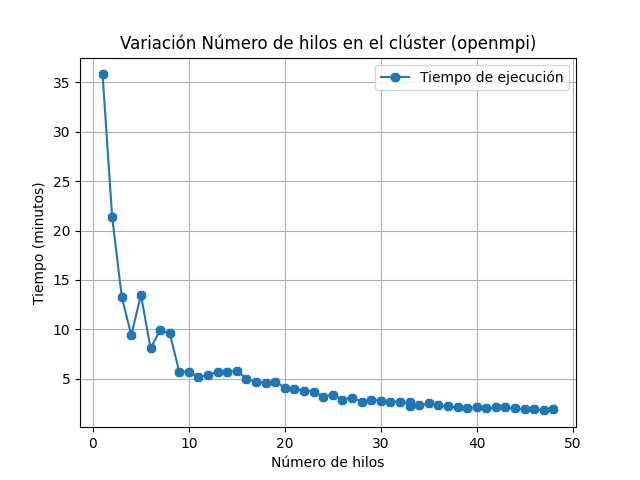
\includegraphics[width=0.9\textwidth]{images/hilos_openmpi.png}
	%caption{\scriptsize{Medición tiempo de ejecución variando el número de hilos en la aplicación}}
	\label{fig:AntennaDesign}
\end{figure}




% \begin{figure}[htb]
% 	\centering
% 	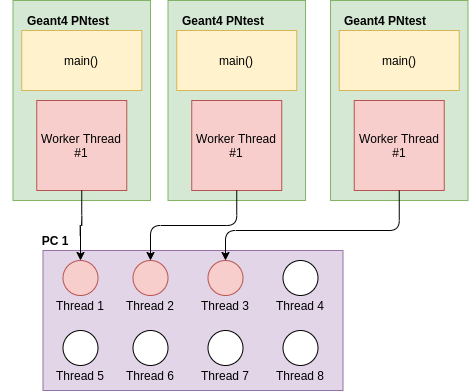
\includegraphics[width=0.5\textwidth]{images/Diagram_hilos_openmpi.png}
% 	%\caption{\scriptsize{Medición tiempo de ejecución variando el número de hilos en la aplicación}}
% 	\label{fig:AntennaDesign}
% \end{figure}





\newpage

\subsection{Comparación Clúster vs 1 PC, variando el número de neutrones}

\begin{itemize}
    \item \textbf{Simulación:} G4pntest
    \item \textbf{Energía:} 0.025 eV
    \item \textbf{Número de neutrones:} \num{200e6}
    \item \textbf{Número de hilos utilizados en PC:} 8 
    \item \textbf{Número de hilos utilizados en el Clúster:} 48
    
\end{itemize}


\begin{table}[H]
\centering
\begin{tabular}{|l|c|c|c|}
\hline
                                      & \textbf{\begin{tabular}[c]{@{}c@{}}PC\\ (Geant4MT)\end{tabular}} & \textbf{\begin{tabular}[c]{@{}c@{}}Clúster\\ (open MPI)\end{tabular}} & \textbf{\begin{tabular}[c]{@{}c@{}}Aceleración\\ Clúster\end{tabular}} \\ \hline
\multicolumn{1}{|c|}{\textbf{Tiempo}} & 1 hora 36 minutos                                                & 42 minutos                                                            & 2.3 veces más rápida                                                   \\ \hline
\end{tabular}
\end{table}

\newpage

\subsection{Comparación Resultados de una simulación usando MT y MPI}
Simulación con $1x10^6$ neutrones disparados directamente al suelo en un cono con apertura angular de 85 grados:

La energía de los neutrones sigue la distribución de la fuente de 252Cf. El detector es un cilindro con dimensiones $5x100$ cm2 alto x diámetro

\begin{itemize}
    \item \textbf{Simulación:} G4pntest
    \item \textbf{Energía:} 0.025 eV
    \item \textbf{Número de neutrones:} \num{1e6}
    \item \textbf{Número de hilos utilizados con MT:} 60 
    \item \textbf{Número de hilos utilizados en el Clúster:} 40
    
\end{itemize}


\begin{figure}[htb]
	\centering
	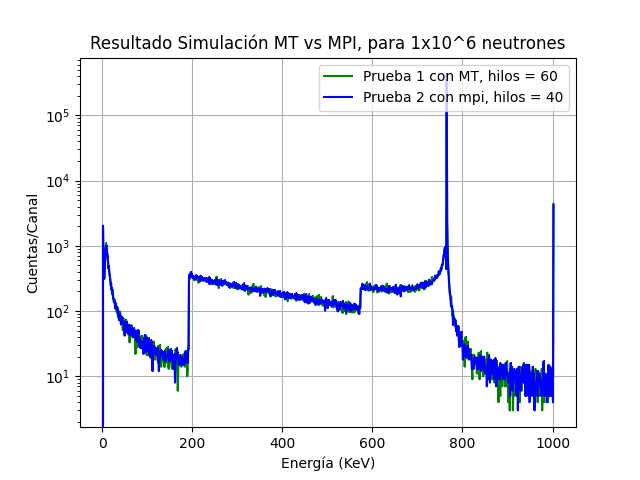
\includegraphics[width=0.9\textwidth]{images/test_MT_vs_Cluster.png}
	%caption{\scriptsize{Medición tiempo de ejecución variando el número de hilos en la aplicación}}
	\label{fig:AntennaDesign}
\end{figure}


%\input{content/08_configSimuMPI.tex}
%\input{content/09_error}
%\input{content/10_avance1.tex}
%\input{content/10_avance2.tex}
%\input{content/10_avance3.tex}



%\section{Bibliografía}

\begin{thebibliography}{}
\bibitem{1} 


\end{thebibliography}


\end{document}



















